\documentclass[tikz]{standalone}

\IfStandalone{\usepackage{mathtools}}{}

\usetikzlibrary{shapes}
\usetikzlibrary{calc} 
\usetikzlibrary{positioning}
\usetikzlibrary{arrows.meta}



% This bascially automates a \newcommand{<name>}{} to ensure
% that a command with the given <name> does not already exist
\providecommand*{\pgfmathsetnewmacro}[2]{%
    \newcommand*{#1}{}% Error if already defined
    \pgfmathsetmacro{#1}{#2}%
}%


\begin{document}
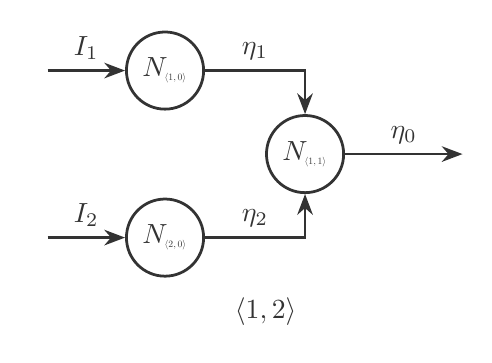
\begin{tikzpicture}[black!80, line width = 1pt]


    \coordinate (O) at (0,0);


    \begin{scope}[on grid]
        
        \node (O) at (2,0) [circle, draw, fill = white] {$N_{\substack{\scalebox{0.35}{${\left\langle 1,1 \right\rangle}$}}}$};

        
        \node (N1) [circle, draw, fill = white, above left=1.5 of O.south west] {$N_{\substack{\scalebox{0.35}{${\left\langle 1,0 \right\rangle}$}}}$};
        \node (N2) [circle, draw, fill = white, below left=1.5 of O.north west] {$N_{\substack{\scalebox{0.35}{${\left\langle 2,0 \right\rangle}$}}}$};

        \node (I1)  [left = 2 of N1.east] {};
        \node (I2)  [left = 2 of N2.east] {};

        
        \draw[-{Stealth}] (N1) -| (O) node [pos=0.25, above] {$\eta_1$};
        \draw[-{Stealth}] (N2) -| (O) node [pos=0.25, above] {$\eta_2$};
        
        \draw[-{Stealth}] (I1) -- (N1) node [midway, above] {$I_1$};
        \draw[-{Stealth}] (I2) -- (N2) node [midway, above] {$I_2$};

        \draw[-{Stealth}] (O) -- +(0:2cm) node [midway, above] {$\eta_0$};
        
        \node at (0,0) [yshift = -2cm , xshift = 1.5cm] {$\left\langle 1,2 \right\rangle$};
    \end{scope}
    
    
    
\end{tikzpicture}
\end{document}